%%%
%
% $Autor: Wings $
% $Date: 2024-10-31 11:15:45Z $
% $File: file.tex $
% $Version: 1 $
%
% Project: 
%
%%%


\chapter{Komplettes System}
\label{chap:komplettes_system}

\section{Beschreibung des Gesamtsystems}
\label{sec:komplettes_system_beschreibung}

Das Gesamtsystem besteht aus einer mechanischen Achskonstruktion, einer elektrischen Leistungsversorgung, einer Mikrocontrollersteuerung und einem thermischen Schneidwerkzeug. 

Die zentrale Funktion des Systems besteht darin, einen elektrisch erwärmten Schneiddraht entlang einer definierten Bahn durch Schaumstoff zu führen. Die Bahnbewegung wird durch Schrittmotoren erzeugt. Die Ansteuerung der Schrittmotoren erfolgt über den Arduino Uno, das CNC Shield V3 und die eingesetzten A4988-Schrittmotortreiber. Der Heißdraht wird getrennt von der Motorsteuerung über ein MOSFET-PWM-Schaltmodul geschaltet.

Die Maschine besitzt damit zwei wesentliche Wirkbereiche. Der erste Bereich ist die Bewegungssteuerung der Achsen. Der zweite Bereich ist die thermische Trennung des Werkstoffs durch den Heißdraht. Beide Bereiche müssen aufeinander abgestimmt werden, da die Schnittqualität sowohl von der Achsbewegung als auch von der Heizleistung abhängt.

Abbildung~\ref{fig:automatisierungssystem_cnc} zeigt den CNC-Heißdrahtschneider als Automatisierungssystem. Die Darstellung trennt Steuerung, Maschine, Signalfluss und Leistungsfluss.

\begin{figure}[H]
	\centering
	\resizebox{0.78\textwidth}{!}{%
		\begin{circuitikz}[x=1cm,y=1cm,>=stealth]
	
	% Grundschrift
	\tikzstyle{every node}=[font=\fontsize{13pt}{16pt}\selectfont]
	
	% Kleine Schrift fuer Pfeilbeschriftungen
	\tikzset{
		pfeiltext/.style={
			font=\fontsize{6.5pt}{8pt}\selectfont,
			fill=white,
			fill opacity=1,
			text opacity=1,
			inner xsep=0.025cm,
			inner ysep=0.015cm,
			align=center
		}
	}
	
	% Gesamtsystem
	\draw [line width=2pt, dashed] (1.0,16.75) rectangle (16.5,-1.125);
	
	\node [
	font=\fontsize{25.0pt}{32.5pt}\selectfont,
	fill=white,
	inner xsep=0.080cm,
	inner ysep=0.085cm,
	rounded corners=0.020cm
	] at (9.125,16) {\textbf{Gesamtsystem}};
	
	% Maschine
	\draw [
	color={rgb,255:red,246; green,27; blue,27},
	draw opacity=1,
	line width=2pt,
	dashed
	] (4.375,6.625) rectangle (14.125,-0.125);
	
	\node [
	font=\fontsize{18.2pt}{23.7pt}\selectfont,
	color={rgb,255:red,253; green,17; blue,17},
	fill=white,
	text opacity=1,
	inner xsep=0.080cm,
	inner ysep=0.085cm,
	rounded corners=0.020cm
	] at (9.125,5.95) {\textbf{Maschine}};
	
	\draw [line width=1.2pt] (5,5.625) rectangle (8,3.5);
	\draw [line width=1.2pt] (10.375,5.625) rectangle (13.25,3.5);
	
	\node [
	font=\fontsize{13.1pt}{17.0pt}\selectfont,
	inner xsep=0.080cm,
	inner ysep=0.085cm,
	rounded corners=0.020cm
	] at (6.5,4.625) {\textbf{Heizdraht}};
	
	\node [
	font=\fontsize{13.1pt}{17.0pt}\selectfont,
	inner xsep=0.080cm,
	inner ysep=0.085cm,
	rounded corners=0.020cm
	] at (11.75,4.5) {\textbf{Motoren}};
	
	% Steuerung
	\draw [
	color={rgb,255:red,14; green,170; blue,248},
	draw opacity=1,
	line width=2pt,
	dashed
	] (4.375,15.25) rectangle (13.875,7.5);
	
	\node [
	font=\fontsize{18.2pt}{23.7pt}\selectfont,
	color={rgb,255:red,95; green,170; blue,242},
	fill=white,
	text opacity=1,
	inner xsep=0.080cm,
	inner ysep=0.085cm,
	rounded corners=0.020cm
	] at (9.125,14.75) {\textbf{Steuerung}};
	
	\draw [line width=1.2pt] (6.75,14.125) rectangle (11.375,13);
	
	\node [
	font=\fontsize{18.2pt}{23.7pt}\selectfont,
	inner xsep=0.080cm,
	inner ysep=0.085cm,
	rounded corners=0.020cm
	] at (9.125,13.5) {\textbf{Computer}};
	
	\draw [line width=1.2pt] (5.125,11.625) rectangle (8,10.25);
	\draw [line width=1.2pt] (10.25,11.625) rectangle (13.125,10.25);
	\draw [line width=1.2pt] (5.125,9.375) rectangle (8,8.125);
	\draw [line width=1.2pt] (10.25,9.375) rectangle (13.125,8.125);
	
	\node [
	font=\fontsize{9.2pt}{11.5pt}\selectfont,
	inner xsep=0.040cm,
	inner ysep=0.040cm,
	rounded corners=0.020cm
	] at (6.5,10.875) {\textbf{Mikrocontroller}};
	
	\node [
	font=\fontsize{9.2pt}{11.5pt}\selectfont,
	inner xsep=0.040cm,
	inner ysep=0.040cm,
	rounded corners=0.020cm
	] at (11.625,10.75) {\textbf{CNC-Shield}};
	
	\node [
	font=\fontsize{10.8pt}{14.1pt}\selectfont,
	inner xsep=0.080cm,
	inner ysep=0.085cm,
	rounded corners=0.020cm
	] at (6.5,8.75) {\textbf{MOSFET}};
	
	\node [
	font=\fontsize{9.2pt}{11.5pt}\selectfont,
	inner xsep=0.040cm,
	inner ysep=0.040cm,
	rounded corners=0.020cm
	] at (11.625,8.625) {\textbf{Motor-Treiber}};
	
	% Sensoren und Bedienelemente
	\draw [line width=1.2pt] (10.375,2.375) rectangle (13.375,0.5);
	
	\node [
	font=\fontsize{13.1pt}{17.0pt}\selectfont,
	inner xsep=0.080cm,
	inner ysep=0.085cm,
	rounded corners=0.020cm
	] at (11.875,1.5) {\textbf{Endschalter}};
	
	\draw [line width=1.2pt] (5,2.375) rectangle (8,0.5);
	
	\node [
	font=\fontsize{11.9pt}{15.5pt}\selectfont,
	inner xsep=0.080cm,
	inner ysep=0.085cm,
	rounded corners=0.020cm
	] at (6.5,1.5) {\textbf{Druckknöpfe}};
	
	% Serielle Kommunikation
	\draw [line width=0.9pt, <->] (7.5,13) -- (7.5,11.625)
	node[
	pos=0.5,
	left,
	pfeiltext
	]{\textbf{serielle}\\\textbf{Kommunikation}};
	
	% Shield Header
	\draw [line width=0.9pt, ->] (8,11.125) -- (10.25,11.125)
	node[
	pos=0.5,
	above,
	pfeiltext
	]{\textbf{Shield-Header}};
	
	% STEP DIR ENABLE
	\draw [line width=0.9pt, ->] (11.625,10.25) -- (11.625,9.375)
	node[
	pos=0.5,
	right,
	pfeiltext
	]{\textbf{STEP, DIR}\\\textbf{ENABLE}};
	
	% Motorstrom
	\draw [line width=0.9pt, ->] (11.75,8.125) -- (11.75,5.625)
	node[
	pos=0.35,
	right,
	pfeiltext
	]{\textbf{Motorstrom}};
	
	% Laststrom
	\draw [line width=0.9pt, ->] (6.375,8.125) -- (6.375,5.625)
	node[
	pos=0.35,
	left,
	pfeiltext
	]{\textbf{Laststrom}};
	
	% PWM-Signal
	\draw [line width=0.9pt, ->] (6.5,10.25) -- (6.5,9.375)
	node[
	pos=0.5,
	right,
	pfeiltext
	]{\textbf{PWM-Signal}};
	
	% Endschalter-Rueckmeldung
	\draw [line width=0.9pt] (11.875,0.5) -- (11.875,0.05);
	\draw [line width=0.9pt] (11.875,0.05) -- (2.15,0.05);
	\draw [line width=0.9pt] (2.15,0.05) -- (2.15,10.95);
	\draw [line width=0.9pt, ->] (2.15,10.95) -- (5.125,10.95);
	
	\node[
	pfeiltext
	] at (3.25,11.35) {\textbf{Endschalter-}\\\textbf{Rückmeldung}};
	
	% Druckknopf-Signal
	\draw [line width=0.9pt] (5,1.5) -- (2.75,1.5);
	\draw [line width=0.9pt] (2.75,1.5) -- (2.75,10.45);
	\draw [line width=0.9pt, ->] (2.75,10.45) -- (5.125,10.45);
	
\node[
pfeiltext
] at (3.35,1.05) {\textbf{digitales}\\\textbf{Eingangssignal}};
	
\end{circuitikz}
	}
	\caption{Schematische Darstellung des CNC-Heißdrahtschneiders als Automatisierungssystem}
	\label{fig:automatisierungssystem_cnc}
\end{figure}

\section{Design und Aufbau}
\label{sec:komplettes_system_design_aufbau}

Der Aufbau ist modular ausgeführt. Die mechanische Baugruppe trägt die Achsen und den Schneiddraht. Die elektrische Baugruppe enthält die Steuer- und Leistungskomponenten. Die Software erzeugt die Steuerbefehle für die Bewegung und stellt die Bedien- beziehungsweise Testfunktionen bereit.

Der Arduino Uno dient als zentrale Steuereinheit. Auf ihm befindet sich das CNC Shield V3, das die Steuerpins des Arduino auf die Anschlüsse der Schrittmotortreiber, Motoren und Endschalter verteilt. Die A4988-Schrittmotortreiber übernehmen die Leistungsansteuerung der Schrittmotoren. Die Motoren bewegen die Achsen der Maschine und führen dadurch den Heißdraht entlang der gewünschten Kontur.

Der Heißdraht wird nicht direkt über den Arduino versorgt. Stattdessen wird ein MOSFET-PWM-Schaltmodul verwendet. Dieses Modul schaltet den Laststrom des Heißdrahts. Der Arduino liefert nur das Steuersignal. Dadurch werden Logikteil und Lastteil funktional getrennt.

Die Spannungsversorgung ist ebenfalls aufgeteilt. Die Motoren und der Heißdraht werden mit einer Nennspannung von \(24\,\mathrm{V}\) versorgt. Der Arduino und die Logiksignale arbeiten mit niedrigeren Spannungen. Für zusätzliche Verbraucher oder Hilfsschaltungen kann ein DC-DC-Abwärtswandler eingesetzt werden.

\section{Hardware-Schnittstellen}
\label{sec:komplettes_system_hardware_schnittstellen}

Die Hardware-Schnittstellen verbinden die einzelnen Baugruppen elektrisch und mechanisch miteinander. Die Signalleitungen übertragen Steuerinformationen. Die Leistungsleitungen versorgen Motoren und Heißdraht.

\begin{table}[H]
	\centering
	\caption{Hardware-Schnittstellen des Gesamtsystems}
	\label{tab:hardware_schnittstellen_gesamtsystem}
	\begin{tabular}{p{4cm} p{4cm} p{6cm}}
		\hline
		\textbf{Schnittstelle} & \textbf{Verbindung} & \textbf{Funktion} \\
		\hline
		Arduino Uno -- CNC Shield V3 & Steckverbindung & Übergabe der digitalen Steuerpins an das Shield \\
		CNC Shield -- A4988 & Treibersteckplätze & Übergabe von STEP-, DIR- und ENABLE-Signalen \\
		A4988 -- Schrittmotor & Motoranschlüsse & Leistungsansteuerung der Motorwicklungen \\
		CNC Shield -- Endschalter & Digitale Eingänge & Erfassung von Referenz- oder Endpositionen \\
		Arduino/CNC Shield -- MOSFET-Modul & PWM-Signal und GND & Ansteuerung der Heißdraht-Leistungsstufe \\
		MOSFET-Modul -- Heißdraht & Lastanschluss & Schalten des Heißdrahtstroms \\
		Netzteil -- CNC Shield & Versorgungsklemme & Motorspannung für die Schrittmotortreiber \\
		Netzteil -- MOSFET-Modul & Versorgungsklemme & Versorgung des Heißdrahtkreises \\
		DC-DC-Wandler -- Zusatzmodule & Versorgungsausgang & Bereitstellung angepasster Hilfsspannungen \\
		\hline
	\end{tabular}
\end{table}

Für alle Signale, die zwischen Steuerung und Leistungsmodulen übertragen werden, ist ein gemeinsamer Massebezug erforderlich. 

\clearpage

\begin{figure}[p]
	\centering
	\vspace*{-2.0cm}
	\makebox[\textwidth][c]{%
		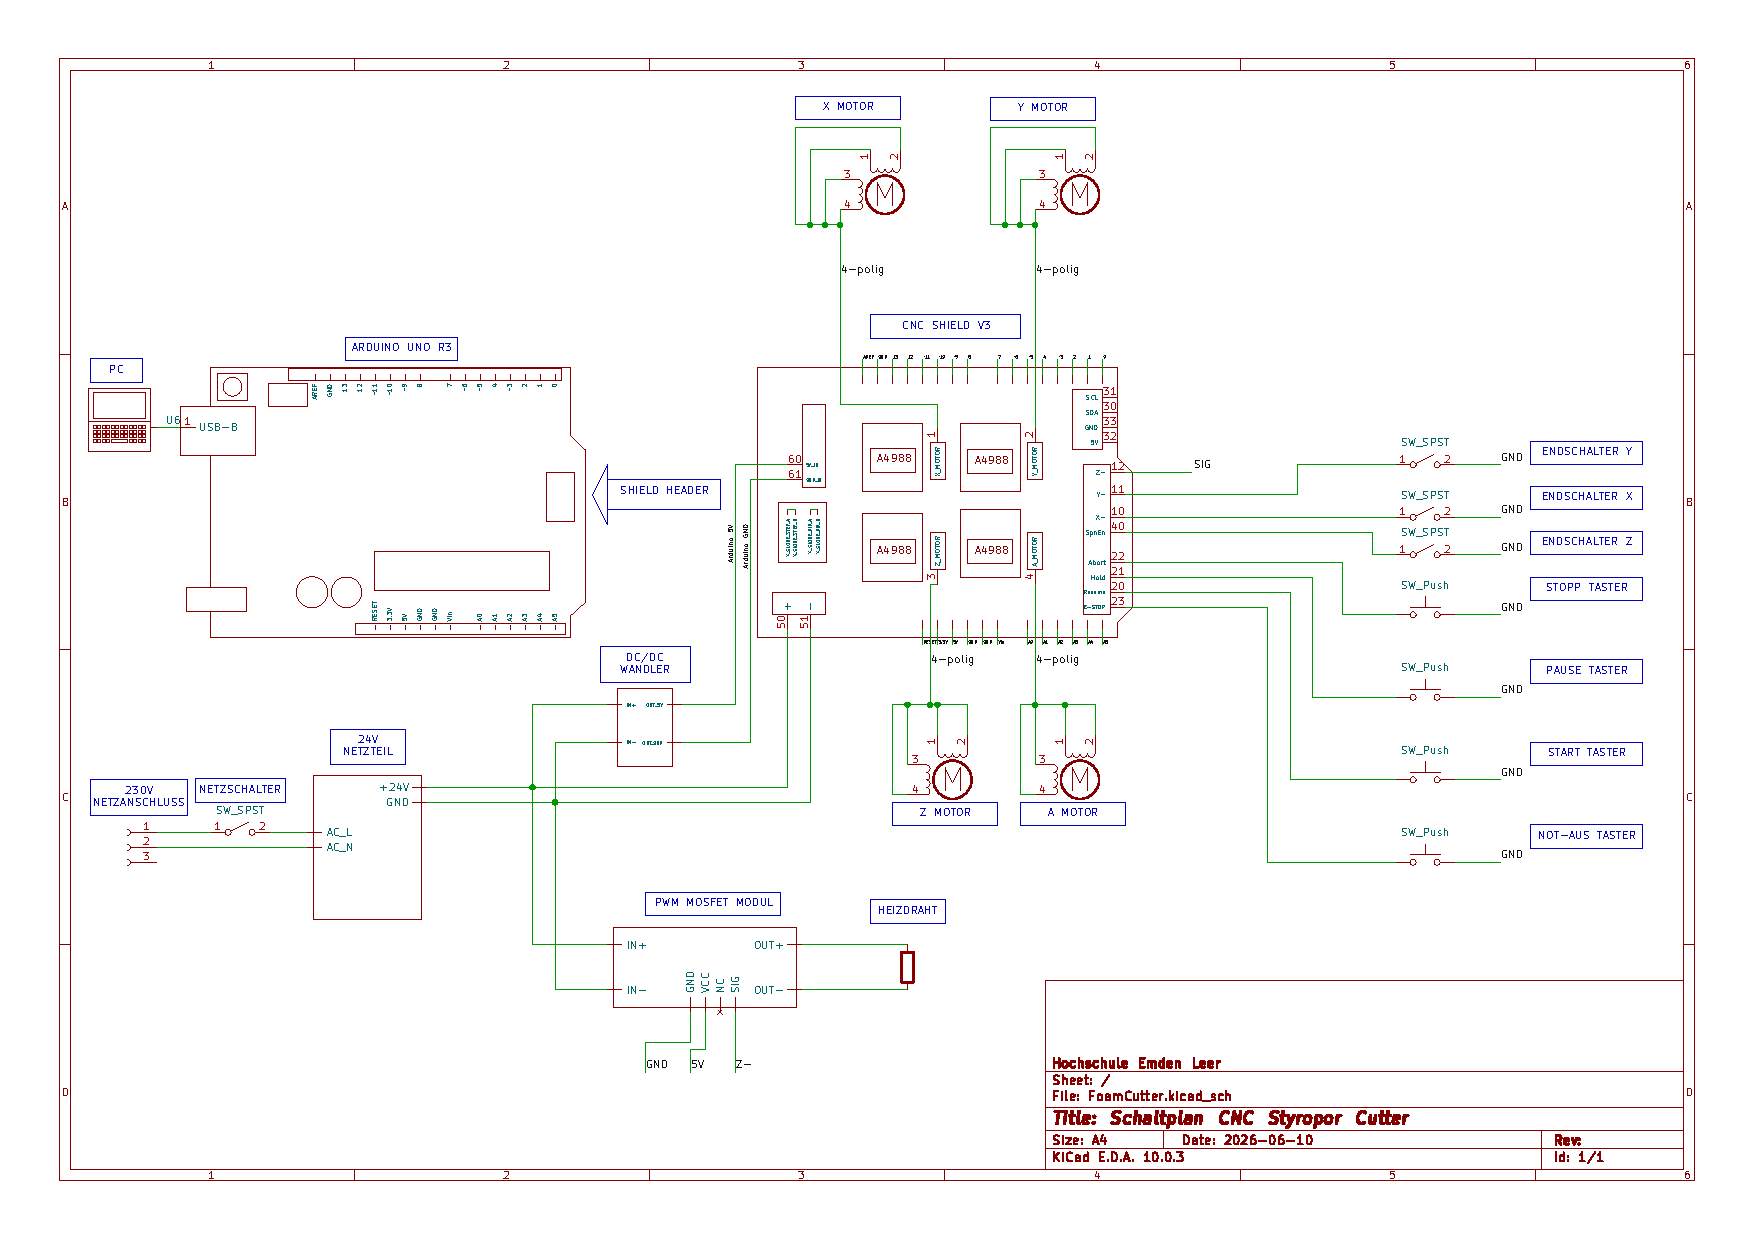
\includegraphics[
		angle=90,
		width=1.08\textheight,
		height=1.55\textwidth,
		keepaspectratio
		]{../../Images/General/FoamCutter.pdf}
	}
	\caption{Schaltplan des CNC-Heißdrahtschneiders}
	\label{fig:schaltplan_foamcutter}
\end{figure}

\clearpage

\section{Eigenschaften des Gesamtsystems}
\label{sec:komplettes_system_eigenschaften}

Das Gesamtsystem besitzt vier mechanische Achsen. Davon werden drei Achsen unabhängig angesteuert. Die A-Achse ist als Y-Klon ausgeführt und bewegt sich synchron zur Y-Achse. Dadurch kann der Heißdraht auf beiden Seiten geführt werden, ohne dass für die zweite Y-Seite eine eigene Bewegungsberechnung notwendig ist.

\begin{table}[H]
	\centering
	\caption{Technische Kenndaten des Gesamtsystems}
	\label{tab:technische_kenndaten_gesamtsystem}
	\begin{tabular}{p{5cm} p{4cm} p{6cm}}
		\hline
		\textbf{Kenngröße} & \textbf{Wert} & \textbf{Bemerkung} \\
		\hline
		Steuerung & Arduino Uno R3 & zentrale Mikrocontrollersteuerung \\
		Firmware & GRBL 1.1h & CNC-Firmware auf dem Arduino Uno R3 \\
		Erweiterungsplatine & CNC Shield V3 & Verteilung der Achs- und Endschaltersignale \\
		Motortreiber & A4988 & Schrittmotortreiber für die Achsantriebe \\
		Anzahl Achsen & 4 & X, Y, Z und A \\
		Unabhängig gesteuerte Achsen & 3 & A-Achse als Y-Klon \\
		Antrieb X/Z & Zahnriemen & Riemensteigung \(2\,\mathrm{mm}\) \\
		Antrieb Y/A & Trapezgewindespindel & Steigung ca. \(2\,\mathrm{mm/U}\) \\
		Riemenscheibe X/Z & 20 Zähne & ergibt \(40\,\mathrm{mm}\) Verfahrweg pro Motorumdrehung \\
		Versorgungsspannung & \(24\,\mathrm{V}\,\mathrm{DC}\) & gemeinsame Nennspannung der Leistungsversorgung \\
		Motorspannung & \(24\,\mathrm{V}\) & Nennwert \\
		Heißdrahtspannung & \(24\,\mathrm{V}\) & Nennwert \\
		Heißdrahtsteuerung & PWM-MOSFET-Modul & Schalten des Heißdrahtkreises \\
		Drahtdurchmesser & \(0{,}4\,\mathrm{mm}\) & Herstellerwert \\
		PWM-Bereich Heißdraht & \(0\)--\(15\,\%\) & verwendeter Einstellbereich \\
		Schnittfugenbreite & ca. \(1\)--\(2\,\mathrm{mm}\) & abhängig von Vorschubgeschwindigkeit und Heizleistung \\
		\hline
	\end{tabular}
\end{table}

Das Gesamtsystem besitzt folgende funktionale Eigenschaften:

\begin{itemize}
	\item rechnergestützte Bewegung des Heißdrahts über Schrittmotorachsen,
	\item getrennte Ansteuerung von Bewegungs- und Heißdrahtkreis,
	\item Verwendung von STEP-, DIR- und ENABLE-Signalen für die Achsantriebe,
	\item Mikroschrittauflösung von \(1/2\) an allen vier Achsen,
	\item Leistungsbeeinflussung des Heißdrahts über ein PWM-MOSFET-Modul,
	\item Referenzfahrt über Endschalter an X-, Y- und Z-Achse,
	\item dauerhafte Motorhaltefunktion über \texttt{\$1 = 255}.
\end{itemize}

Die Genauigkeit des Systems hängt nicht nur von den elektronischen Komponenten ab. Auch mechanische Faktoren wie Achsspiel, Reibung, Drahtspannung und Rahmensteifigkeit beeinflussen das Ergebnis. Zusätzlich wirken thermische Prozessgrößen wie Heißleistung, Vorschubgeschwindigkeit und Materialdicke auf die Schnittqualität.

\section{Software-Schnittstellen}
\label{sec:komplettes_system_software_schnittstellen}

Die Programmierung und Inbetriebnahme erfolgen über einen Computer mit Arduino IDE. Der Arduino Uno wird über USB mit dem Computer verbunden. Über diese Verbindung werden Programme auf den Mikrocontroller übertragen. Zusätzlich kann die serielle Schnittstelle zur Ausgabe von Status- und Testinformationen verwendet werden.

Für den CNC-Betrieb wird GRBL 1.1h verwendet. Die Firmware verarbeitet Bewegungsbefehle und erzeugt daraus die STEP-, DIR- und ENABLE-Signale für die Schrittmotortreiber. Für Funktionstests können zusätzlich einfache Arduino-Sketches eingesetzt werden, mit denen einzelne Baugruppen wie Motoren, Endschalter, OLED-Anzeige oder Heißdraht separat geprüft werden.

Für einen CNC-nahen Betrieb können Bewegungsdaten in Form von G-Code oder vergleichbaren Koordinateninformationen verwendet werden. Dabei beschreibt die Software Zielpositionen, Bewegungsrichtungen und Vorschubgeschwindigkeiten. Die Steuerung muss diese Daten in zeitlich koordinierte Schrittimpulse für die Achsen umsetzen.

Die softwareseitigen Schnittstellen:

\begin{itemize}
	\item USB-Verbindung zwischen Computer und Arduino,
	\item serielle Kommunikation zur Übertragung von Programm- und Statusdaten,
	\item GRBL 1.1h als Firmware zur Bewegungssteuerung,
	\item digitale Ausgangssignale für STEP, DIR und ENABLE,
	\item PWM-Ausgang zur Ansteuerung des MOSFET-Schaltmoduls,
	\item digitale Eingangssignale der Endschalter.
\end{itemize}

\section{Installation des Gesamtsystems}
\label{sec:komplettes_system_installation}

Die Installation beginnt mit der mechanischen Montage des Rahmens, der Achsen und der Drahtführung. Der Schneiddraht wird mechanisch befestigt und gespannt. Dabei muss geprüft werden, ob der Draht frei durch den Arbeitsbereich geführt werden kann und nicht an Bauteilen schleift.

Anschließend werden Arduino Uno und CNC Shield montiert. Die A4988-Schrittmotortreiber werden in die vorgesehenen Steckplätze des Shields eingesetzt. Dabei muss auf die korrekte Ausrichtung der Treibermodule geachtet werden. Eine falsche Orientierung kann die Treiber beschädigen.

Danach werden die Schrittmotoren an die Motoranschlüsse des CNC Shields angeschlossen. Die Endschalter werden mit den vorgesehenen Eingängen verbunden. Das MOSFET-PWM-Schaltmodul wird mit dem Steuersignal, Masse und dem Heißdrahtkreis verbunden. Abschließend werden die Spannungsversorgung für Motoren, Logik und Heißdraht geprüft.

Vor dem ersten Betrieb dürfen Motor- und Heißdrahtversorgung noch nicht dauerhaft aktiv betrieben werden. Zuerst müssen alle Leitungen, Steckverbindungen, Polaritäten und Masseverbindungen kontrolliert werden.

\section{Konfiguration}
\label{sec:komplettes_system_konfiguration}

Nach der Installation wird das System konfiguriert. Zuerst wird die Arduino IDE eingerichtet und das verwendete Board ausgewählt. Danach wird der passende Port eingestellt und die Firmware beziehungsweise ein Testsketch übertragen.

Die Schrittmotortreiber müssen vor dem Betrieb eingestellt werden. Besonders wichtig ist die Strombegrenzung. Eine zu hohe Einstellung kann zu starker Erwärmung oder zur Abschaltung des Treibers führen. Eine zu niedrige Einstellung kann Schrittverluste verursachen. Die Mikroschrittauflösung ist an allen vier Achsen auf \(1/2\) eingestellt.

\begin{table}[H]
	\centering
	\caption{GRBL- und Bewegungsparameter des Gesamtsystems}
	\label{tab:grbl_bewegungsparameter_gesamtsystem}
	\begin{tabular}{p{5cm} p{4cm} p{6cm}}
		\hline
		\textbf{Parameter} & \textbf{Wert} & \textbf{Bemerkung} \\
		\hline
		Firmware & GRBL 1.1h & CNC-Firmware auf dem Arduino Uno R3 \\
		Schritte pro Millimeter X & \texttt{\$100 = 10} & Kalibrierwert X-Achse \\
		Schritte pro Millimeter Y & \texttt{\$101 = 50} & Kalibrierwert Y-Achse \\
		Schritte pro Millimeter Z & \texttt{\$102 = 10} & Kalibrierwert Z-Achse \\
		Schritte pro Millimeter A & 50 & A-Achse als Y-Klon \\
		Maximale Verfahrgeschwindigkeit X & \(2000\,\mathrm{mm/min}\) & GRBL-Wert für X-Achse \\
		Maximale Verfahrgeschwindigkeit Y & \(2000\,\mathrm{mm/min}\) & GRBL-Wert für Y-Achse \\
		Maximale Verfahrgeschwindigkeit Z & \(2000\,\mathrm{mm/min}\) & GRBL-Wert für Z-Achse \\
		Beschleunigung X/Y/Z & \(30\,\mathrm{mm/s^2}\) & eingestellter Beschleunigungswert \\
		Motorhaltefunktion & \texttt{\$1 = 255} & Motoren bleiben dauerhaft bestromt \\
		
		\hline
	\end{tabular}
\end{table}

Die Achsen wurden mit den angegebenen Schritten pro Millimeter kalibriert. Der rechnerische Wert wird durch Messfahrten überprüft. Wenn die gemessene Strecke vom Sollwert abweicht, muss der Schrittwert angepasst werden.

Auch die Heißdrahtleistung muss eingestellt werden. Dazu wird die PWM-Ansteuerung zunächst mit niedriger Leistung getestet. Der verwendete Einstellbereich liegt bei \(0\)--\(15\,\%\). Danach werden Probeschnitte durchgeführt, um Heizleistung und Vorschubgeschwindigkeit aufeinander abzustimmen.

Die Referenzfahrt ist vorhanden und aktiviert. Es werden drei Endschalter für X-, Y- und Z-Achse eingesetzt. Die Referenzposition liegt oben und hinten.

\section{Daten, Strukturen und Typen}
\label{sec:komplettes_system_daten}

Im Gesamtsystem werden verschiedene Daten und Parameter verwendet. Sie beschreiben die Achsbewegung, die elektrische Ansteuerung und die Bewertung des Schneidprozesses.

\begin{table}[H]
	\centering
	\caption{Daten und Parameter des Gesamtsystems}
	\label{tab:daten_parameter_gesamtsystem}
	\begin{tabular}{p{4cm} p{4cm} p{6cm}}
		\hline
		\textbf{Parameter} & \textbf{Wert/Typ} & \textbf{Bedeutung} \\
		\hline
		Schrittzahl & Ganzzahl & Anzahl der ausgegebenen STEP-Impulse \\
		Richtung & digitaler Zustand & Bewegungsrichtung einer Achse über DIR \\
		Mikroschrittauflösung & \(1/2\) & Einstellung an allen vier Achsen \\
		Vorschubgeschwindigkeit & \(2000\,\mathrm{mm/min}\) & verwendete beziehungsweise maximale Verfahrgeschwindigkeit \\
		Schritte pro Millimeter & X: 10, Y: 50, Z: 10, A: 50 & Umrechnung zwischen Steuerimpulsen und realem Verfahrweg \\
		PWM-Wert Heißdraht & \(0\)--\(15\,\%\) & Tastverhältnis zur Beeinflussung der Heizleistung \\
		Endschalterzustand & digitaler Eingangswert & Erkennung der Referenzposition \\
		Drahtdurchmesser & \(0{,}4\,\mathrm{mm}\) & Herstellerwert des Schneiddrahts \\
		Schnittfugenbreite & ca. \(1\)--\(2\,\mathrm{mm}\) & Bewertungsgröße für die Schnittqualität \\
		Werkstückabmessung & Messwert & Vergleich zwischen Soll- und Ist-Kontur \\
		\hline
	\end{tabular}
\end{table}



\section{Einschränkungen und offene Punkte}
\label{sec:komplettes_system_einschraenkungen_todos}

Das System besitzt mehrere Einschränkungen, die beim Betrieb berücksichtigt werden müssen. Die verwendeten Schrittmotoren arbeiten im einfachen Aufbau ohne direkte Positionsrückmeldung. Die Steuerung erkennt daher nicht automatisch, ob ein Motor Schritte verliert. Schrittverluste müssen durch geeignete Parameter, leichtgängige Mechanik und Funktionstests vermieden werden.

Die Heißdrahttemperatur wird nicht gemessen. Die Einstellung erfolgt über die elektrische Ansteuerung und die Bewertung der Probeschnitte. Dadurch ist die Heizleistung material- und erfahrungsabhängig. Unterschiedliche Schaumstoffarten oder Materialdicken können andere Einstellungen erfordern.

Weitere offene Punkte sind:

\begin{itemize}
	\item Maschinengewicht messen und dokumentieren,
	\item Leistungsaufnahme im Betrieb messen und dokumentieren,
	\item endgültige Standardwerte für Vorschub und PWM für verschiedene Materialien festlegen,
	\item Wiederholgenauigkeit über mehrere Schnitte prüfen,
	\item direkte Temperatur- oder Strommessung am Heißdraht ergänzen,
	\item Kabelführung und Zugentlastung weiter verbessern,
	\item Schutzabdeckung für heiße und bewegte Bereiche ergänzen.
\end{itemize}

\section{Abmaße}
\label{sec:komplettes_system_abmasse}

Die Abmaße des Gesamtsystems ergeben sich aus dem mechanischen Rahmen, dem nutzbaren Arbeitsbereich und der Anordnung der elektrischen Baugruppen. Dabei ist zwischen Außenmaß, Arbeitsbereich und Drahtspannweite zu unterscheiden.

\begin{table}[H]
	\centering
	\caption{Abmaße des Gesamtsystems}
	\label{tab:abmasse_gesamtsystem}
	\begin{tabular}{p{5cm} p{4cm} p{6cm}}
		\hline
		\textbf{Größe} & \textbf{Wert} & \textbf{Bemerkung} \\
		\hline
		Gesamtlänge & \(650\,\mathrm{mm}\) & Außenmaß der Maschine \\
		Gesamtbreite & \(707\,\mathrm{mm}\) & Außenmaß der Maschine \\
		Gesamthöhe & \(583\,\mathrm{mm}\) & Außenmaß einschließlich Drahtführung \\
		Nutzbarer Arbeitsbereich X & \(345\,\mathrm{mm}\) & maximaler Verfahrweg beziehungsweise maximale Werkstückbreite \\
		Nutzbarer Arbeitsbereich Y & \(390\,\mathrm{mm}\) & maximaler Verfahrweg beziehungsweise maximale Werkstückhöhe \\
		Freie Drahtlänge & min. \(450\,\mathrm{mm}\), max. \(688\,\mathrm{mm}\) & freie Länge des gespannten Schneiddrahts \\
		Grundplattenmaß & \(537\,\mathrm{mm} \times 457\,\mathrm{mm}\) & Abmessung der Montage- oder Arbeitsplatte \\
		Maschinengewicht & noch zu messen & offener Messwert \\
		Leistungsaufnahme & noch zu messen & offener Messwert im Betrieb \\
		\hline
	\end{tabular}
\end{table}

Die maximale Werkstückbreite beträgt ca. \(345\,\mathrm{mm}\). Die maximale Werkstückhöhe beträgt ca. \(390\,\mathrm{mm}\). Die maximale Drahtspannweite beträgt \(688\,\mathrm{mm}\). Diese Werte begrenzen den nutzbaren Arbeitsraum der Maschine.

\section{Schlussfolgerung}
\label{sec:komplettes_system_schlussfolgerung}

Das Gesamtsystem verbindet die zuvor beschriebenen Einzelkomponenten zu einem funktionsfähigen CNC-Heißdrahtschneider. Der Arduino Uno übernimmt die Steuerlogik, das CNC Shield verteilt die Achssignale, die A4988-Treiber versorgen die Schrittmotoren und das MOSFET-PWM-Schaltmodul schaltet den Heißdrahtkreis. Die mechanische Baugruppe führt den Draht entlang der gewünschten Kontur.

Ein einsatzfähiger Zustand liegt vor, wenn die Achsen reproduzierbar verfahren, der Heißdraht kontrolliert erwärmt wird, die Endschalter zuverlässig reagieren und Probeschnitte eine nachvollziehbare Schnittqualität zeigen. Die abschließende Bewertung erfolgt daher nicht nur über elektrische Funktionstests, sondern über das reale Schneidergebnis am Werkstück.
